%%% LaTeX Template: Article/Thesis/etc. with colored headings and special fonts
%%%
%%% Source: http://www.howtotex.com/
%%% Feel free to distribute this template, but please keep to referal to http://www.howtotex.com/ here.
%%% February 2011
%%%
%%% Modified January 2016 by CDM

%%%  Preamble
\documentclass[11pt,letterpaper]{article}
\usepackage[margin=1.0in]{geometry}
\usepackage[T1]{fontenc}
\usepackage[bitstream-charter]{mathdesign}
\usepackage[latin1]{inputenc}					
\usepackage{amsmath}						
\usepackage{xcolor}
\usepackage{cite}
\usepackage{hyphenat}
\usepackage{graphicx}
\usepackage{float}
\usepackage{subfigure}
\usepackage{sectsty}
\usepackage[compact]{titlesec} 
\usepackage[tablegrid]{vhistory}
\usepackage{pbox}
\allsectionsfont{\color{accentcolor}\scshape\selectfont}

%%% Definitions
\definecolor{accentcolor}{rgb}{0.0,0.0,0.5} 
\newcommand{\teamname}{Team Mercury}
\newcommand{\productname}{ARGOOSE-Counter Drone Tracking}
\newcommand{\coursename}{CSE 4316: Senior Design I}
\newcommand{\semester}{Fall 2022}
\newcommand{\docname}{Architectural Design Specification}
\newcommand{\department}{Department of Computer Science \& Engineering}
\newcommand{\university}{The University of Texas at Arlington}
\newcommand{\authors}{James Grumbles \\ Nirdesh Sakh \\ Augustine Nguyen \\ Sanyogita Piya \\ Mahin Roddur}

%%% Headers and footers
\usepackage{fancyhdr}
	\pagestyle{fancy}						% Enabling the custom headers/footers
\usepackage{lastpage}	
	% Header (empty)
	\lhead{}
	\chead{}
	\rhead{}
	% Footer
	\lfoot{\footnotesize \teamname \ - \semester}
	\cfoot{}
	\rfoot{\footnotesize page \thepage\ of \pageref{LastPage}}	% "Page 1 of 2"
	\renewcommand{\headrulewidth}{0.0pt}
	\renewcommand{\footrulewidth}{0.4pt}

%%% Change the abstract environment
\usepackage[runin]{abstract}			% runin option for a run-in title
%\setlength\absleftindent{30pt}			% left margin
%\setlength\absrightindent{30pt}		% right margin
\abslabeldelim{\quad}	
\setlength{\abstitleskip}{-10pt}
\renewcommand{\abstractname}{}
\renewcommand{\abstracttextfont}{\color{accentcolor} \small \slshape}	% slanted text

%%% Start of the document
\begin{document}

%%% Cover sheet
{\centering \huge \color{accentcolor} \sc \textbf{\department \\ \university} \par}
\vspace{1 in}
{\centering \huge \color{accentcolor} \sc \textbf{\docname \\ \coursename \\ \semester} \par}
\vspace{0.5 in}
\begin{figure}[h!]
	\centering
   	
\includegraphics[width=0.60\textwidth]{images/Logo (1) (1).PNG}
\end{figure}
\vspace{0.5 in}
{\centering \huge \color{accentcolor} \sc \textbf{\teamname \\ \productname} \par}
\vspace{0.5 in}
{\centering \large \sc \textbf{\authors} \par}
\newpage


%\vspace{1 in}
%\centerline{January 13th, 2012}
%\newpage

%%% Revision History
\begin{versionhistory}
  	\vhEntry{0.1}{10.31.2022}{AN}{first draft}
  	\vhEntry{0.2}{11.13.2022}{AN|JG|SP|NS|MR}{complete draft}
\end{versionhistory}
\newpage

%%% Table of contents
\setcounter{tocdepth}{2}
\tableofcontents
\newpage

%%% List of figures and tables (optional)
\listoffigures
\listoftables
\newpage

%%% Document sections
\section{Introduction}
Your introduction should describe your product concept in sufficient detail that the architectural design will be easy to follow. The introduction may include information used in the first sections of your SRS for this purpose. At a minimum, ensure that the product concept, scope and key requirements are described.
\newpage
\section{System Overview}
This section should describe the overall structure of your software system. Think of it as the strategy for how you will build the system. An architectural "layer" is the top-level logical view, or an abstraction, of your design. Layers should be composed of related elements of similar capabilities, and should be highly independent of other layers, but should have very clearly defined interfaces and interactions with other layers. Each layer should be identified individually and should be unique as to its function and purpose within the system. This section should also contain the high-level block diagram of the layers, as shown in the example below, as well as detailed descriptions of the functions of each layer.

\begin{figure}[h!]
	\centering
 	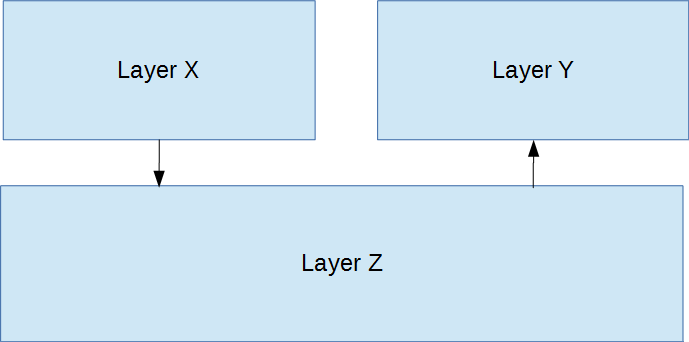
\includegraphics[width=0.60\textwidth]{images/layers}
 \caption{A simple architectural layer diagram}
\end{figure}

\subsection{Layer X Description}
Each layer should be described separately in detail. Descriptions should include the features, functions, critical interfaces and interactions of the layer. The description should clearly define the services that the layer provides. Also include any conventions that your team will use in describing the structure: naming conventions for layers, subsystems, modules, and data flows; interface specifications; how layers and subsystems are defined; etc. 

\subsection{Layer Y Description}
Each layer should be described separately in detail. Descriptions should include the features, functions, critical interfaces and interactions of the layer. The description should clearly define the services that the layer provides. Also include any conventions that your team will use in describing the structure: naming conventions for layers, subsystems, modules, and data flows; interface specifications; how layers and subsystems are defined; etc. 

\subsection{Layer Z Description}
Each layer should be described separately in detail. Descriptions should include the features, functions, critical interfaces and interactions of the layer. The description should clearly define the services that the layer provides. Also include any conventions that your team will use in describing the structure: naming conventions for layers, subsystems, modules, and data flows; interface specifications; how layers and subsystems are defined; etc. 
\newpage
\section{Subsystem Definitions \& Data Flow}
This section breaks down your layer abstraction to another level of detail. Here you grapically represent the logical subsytems that compose each layer and show the interactions/interfaces between those subsystems. A subsystem can be thought of as a programming unit that implements one of the major functions of the layer. It, therefore, has data elements that serve as source/sinks for other subsystems. The logical data elements that flow between subsystems need to be explicitly defined at this point, beginning with a data flow-like diagram based on the block diagram.

\begin{figure}[h!]
	\centering
 	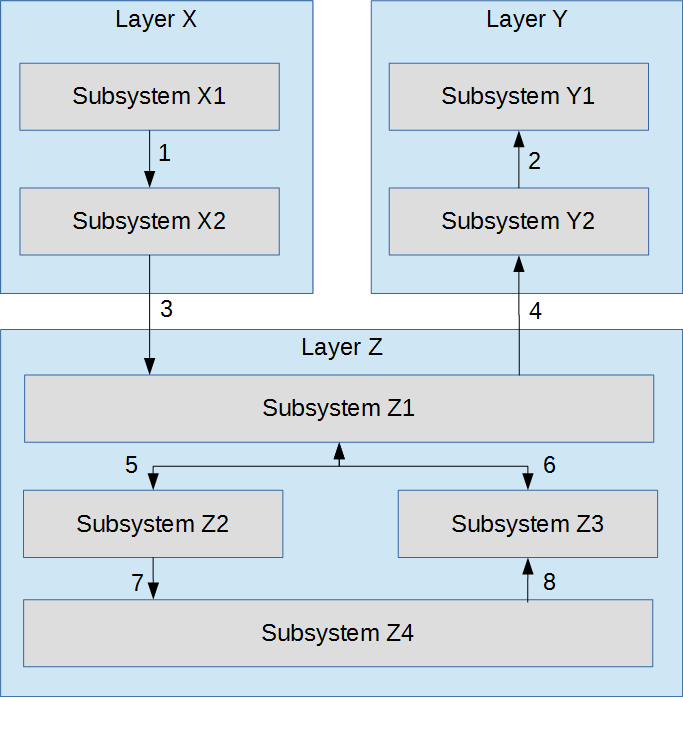
\includegraphics[width=\textwidth]{images/data_flow}
 \caption{A simple data flow diagram}
\end{figure}

\newpage
\section{Detection Layer Subsystems}
The detection layer is the interface between the real-world and the system.  Its subsystems consists of sensors and these sensors take in data such as audio, and then is sent to the processing layer.  It is also controlled by the raspberry pi subsystem in the controller layer.

\subsection{Acoustic Array}
The acoustic array will consist of a hexagonal printed circuit board with six microphones located at each point of the hexagon. Internally the board will contain the audio to digital converter and be capable of processing the microphone inputs from the array and forwarding that information to a digital component for processing. These requirements are meant by a COTS device called ReSpeaker, which will be the component used to meet these requirements. The subsystem will detect audio inputs from the environment and forward the raw analog audio data to the ADC for processing.

\begin{figure}[h!]
	\centering
 	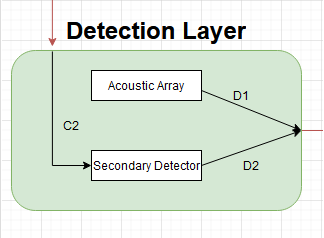
\includegraphics[width=0.50\textwidth]{images/detection}
 \caption{Acoustic Array}
\end{figure}

\subsubsection{Assumptions}
The ReSpeaker will detect across all six microphones and information will be compiled and properly forwarded to the ADC

\subsubsection{Responsibilities}
The subsystems sole purpose is to process raw audio data from the surrounding environment and compile it into a usable data stream. Each microphone works in tandem with the others to generate positional data, then forwards this information to the ADC to process and push further along the pipeline.

\subsubsection{Subsystem Interfaces}

\begin {table}[H]
\caption {Subsystem interfaces} 
\begin{center}
    \begin{tabular}{ | p{1cm} | p{6cm} | p{3cm} | p{3cm} |}
    \hline
    ID & Description & Inputs & Outputs \\ \hline
    \#RS01 & ReSpeaker Microphone Array & \pbox{3cm}{Microphone 1 \\ Microphone 2 \\ Microphone 3 \\ Microphone 4 \\ Microphone 5 \\  Microphone 6} & \pbox{3cm}{Compiled Audio Data to ADC}  \\ \hline
    \#RS02 & Power Supply & \pbox{3cm}{Power In} & \pbox{3cm}{N/A}  \\ \hline
    \end{tabular}
\end{center}
\end{table}

\subsection{Secondary Detector}
The secondary detector is instructed to activate by the raspberry pi when certain conditions are met; once it is activated, the data collected is sent to the ADC for analog to digital conversion.

\begin{figure}[h!]
	\centering
 	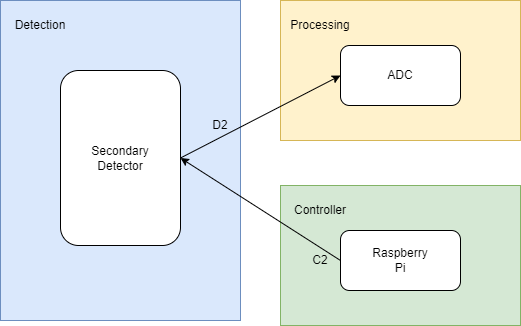
\includegraphics[width=0.60\textwidth]{images/secondary_detector_diagram.drawio}
 \caption{describes secondary detector's relation with the rest of the system}
\end{figure}

\subsubsection{Assumptions}
The secondary detector takes in some sort of sensory detail.  As of yet, this detail has not been determined 100\% yet; however, it will most likely be either some form of frequency detector or a visual detector.  If the secondary detector is to report to ODAS, then the sensory detail would be auditory.

\subsubsection{Responsibilities}
The main responsibility of the secondary detector is to be an extra method of detection, adding to the precision and accuracy.  It is on the standby of the raspberry pi and is processed the same way as the acoustic array.

\subsubsection{Subsystem Interfaces}
\begin {table}[H]
\caption {Subsystem interfaces} 
\begin{center}
    \begin{tabular}{ | p{1cm} | p{6cm} | p{4cm} | p{4cm} |}
    \hline
    ID & Description & Inputs & Outputs \\ \hline
    \#C2 & Activation of Secondary Detector & \pbox{3cm}{Raspberry pi signaling activation} & \pbox{3cm}{Secondary Detector activated}  \\ \hline
    \#D2 & Secondary Detector Data Sending & \pbox{3cm}{Analog data collected} & \pbox{3cm}{Data is sent to the ADC for digital conversion}  \\ \hline
    \end{tabular}
\end{center}
\end{table}
\newpage
\section{Processing Layer Subsystems}
The processing layer takes in analog data, digitizes it, and then processes it.  This processed data is then sent to the controller layer.

\subsection{Analog to Digital Converter (ADC)}
The subsystem ADC's main purpose is to convert real-world-analog data and convert it to digital information, ready to be processed.  The data that gets fed to ADC comes from the detection layer, with its acoustic array and secondary detector subsystems.  Once the ADC has received and converted the data, it transfers the information within its very own processing layer, to the ODAS and secondary processor subsystems.

\begin{figure}[h!]
	\centering
 	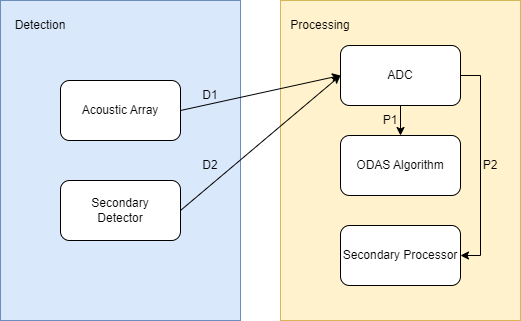
\includegraphics[width=0.60\textwidth]{images/adc_diagram.drawio}
 \caption{describes the relation of ADC along with other subsystems and layers}
\end{figure}

\subsubsection{Assumptions}
The data collected from analog sensors is understood by the ADC and is able to be converted, and the converted digital data is able to be interpreted and processed by the ODAS algorithm and the secondary processor. 

\subsubsection{Responsibilities}
The ADC subsystem is responsible for connecting the real world with the digital system of the product.  The detection layer wouldn't be able to produce any results without its data being processable, and the other subsystems in the processing layer wouldn't have any data to process. 

\subsubsection{Subsystem Interfaces}
\begin {table}[H]
\caption {Subsystem interfaces} 
\begin{center}
    \begin{tabular}{ | p{2cm} | p{6cm} | p{4cm} | p{4cm} |}
    \hline
    ID & Description & Inputs & Outputs \\ \hline
    \#D1/D2 & Analog Data Input & \pbox{3cm}{Acoustic Data \\ Secondary Detector Data} & \pbox{3cm}{Digitized Data}  \\ \hline
    \#P1 & Sending to ODAS & \pbox{3cm}{N/A} & \pbox{3cm}{Digitized Data}  \\ \hline
    \#P2 & Sending to Secondary Processor & \pbox{3cm}{N/A} & \pbox{3cm}{Digitized Data}  \\ \hline
    \end{tabular}
\end{center}
\end{table}

\subsection{ODAS Algorithm}
ODAS is an open source software developed for taking in multiple audio data sources and compiling it into usable data streams. For the purposes of the ARGOOSE system, ODAS will utilize a modified sourcing code to locate the sound of drones that are detected within the area of operation. At default, ODAS detects raw sounds and locations based off of the ReSpeaker array. This information is compiled and displayed on the software to pinpoint location and event data. Data streams will come in from the ADC on detected sound patterns, will be identified and manipulated by ODAS and then forwarded on to the Raspberry pi controller to display and interpret relevant data.

\begin{figure}[h!]
	\centering
 	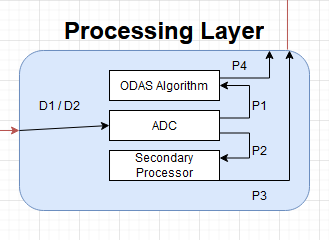
\includegraphics[width=0.50\textwidth]{images/processing}
 \caption{Example subsystem description diagram}
\end{figure}

\subsubsection{Assumptions}
ODAS algorithmic data processing will accurately detail drone detection and forward data streams that are relevant and interpretable by the Raspberry Pi.
Information received from the ADC will be in a format that is accurately analyzable by the ODAS algorithm.

\subsubsection{Responsibilities}
ODAS is responsible for generating the positional and occurrence data from the raw data stream of the ADC. It is the key component is generating the sample necessary for the controller to determine when and where drone detections should occur.

\subsubsection{Subsystem Interfaces}

\begin {table}[H]
\caption {Subsystem interfaces} 
\begin{center}
    \begin{tabular}{ | p{1cm} | p{6cm} | p{3cm} | p{3cm} |}
    \hline
    ID & Description & Inputs & Outputs \\ \hline
    \#RS01 & ODAS Algorithm & \pbox{3cm}{ADC Data Stream} & \pbox{3cm}{Compiled Detection Data to Controller}  \\ \hline
    \end{tabular}
\end{center}
\end{table}

\subsection{Secondary Processing Subsystem}
The secondary processing subsystem is responsible for activation of the secondary sensors and detection system after the object is suspected to be a drone.

\begin{figure}[h!]
	\centering
 	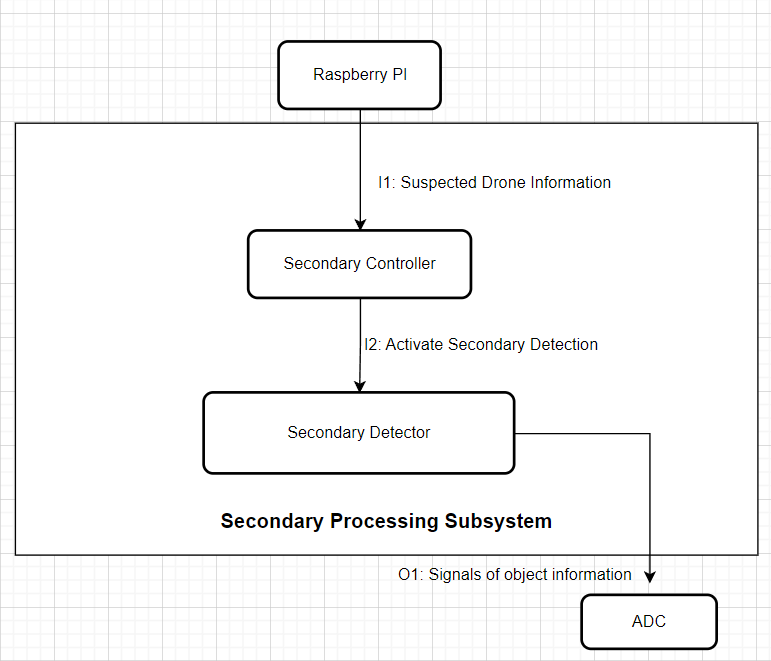
\includegraphics[width=0.60\textwidth]{images/Secondary Processing_Subsystem.png}
 \caption{Secondary Processing Subsystem}
\end{figure}

\subsubsection{Assumptions}
This subsystem assumes that it has an object that is potentially a drone and this information is given by the raspberry pi. 

\subsubsection{Responsibilities}
The primary responsibility of this subsystem is to confirm that the object is a drone. It activates the secondary detection sensors which sends the signals to ADC and these signals are sent through ODAS algorithm to the raspberry pi.

\subsubsection{Subsystem Interfaces}

\begin {table}[H]
\caption {Subsystem interfaces} 
\begin{center}
    \begin{tabular}{ | p{1cm} | p{6cm} | p{3cm} | p{3cm} |}
    \hline
    ID & Description & Inputs & Outputs \\ \hline
    \#I1 & Secondary Controller & \pbox{3cm}{Drone Information} & \pbox{3cm}{Signal to secondary detector}  \\ \hline
    \#I2 & Secondary detector & \pbox{3cm}{Activate secondary sensor} & \pbox{3cm}{N/A}  \\ \hline
    \end{tabular}
\end{center}
\end{table}
\newpage
\section{Controller Layer Subsystems}
The controller layer holds the raspberry pi and drone database subsystem.  The raspberry pi controls much of the system's features, as well as acting as an interface between the different layers.  The drone database holds all the processed data and sends the information to users.

\begin{figure}[h!]
	\centering
 	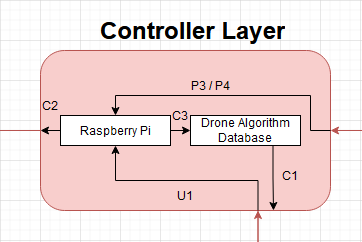
\includegraphics[width=0.50\textwidth]{images/controller.png}
 \caption{Controller subsystems diagram}
\end{figure}

\subsection{Raspberry Pi}
In this system, the Raspberry Pi acts as the central hub that controls the traffic of data flow from one subsystem to another. It also activates functions of specific subsystems based on feedback from another subsystem.

\subsubsection{Assumptions}
The Raspberry Pi is assumed to be powered on throughout the active run time of the system. In addition to that, the Pi needs to have a persistent forms of connections with the other subsystems.

\subsubsection{Responsibilities}
Here is an overview of the data flow pathways that Pi is involved in:
\begin{itemize}
  \item After receiving a positive signal of drone detection from ODAS (which is in the Processing Subsystem), the Pi activates the secondary detector in the Detection Subsystem. 
  \item After receiving confirmation of drone detection from Secondary Processor, it relays relevant drone data to the Drone Algorithm Database.
  \item The Pi also has a bi-directional connection with I/O Subsystems, particularly with the Application subsystem. It is the point of contact in terms of setting updates and user-logins for the user of the system.
\end{itemize}

\subsubsection{Subsystem Interfaces}
Each of the inputs and outputs for the subsystem are defined here. 

\begin {table}[H]
\caption {Raspberry Pi Interfaces} 
\begin{center}
    \begin{tabular}{ | p{2cm} | p{5cm} | p{3cm} | p{4cm} |}
    \hline
    ID & Description & Inputs & Outputs \\ \hline
    \#P4 and C2 & Activation of secondary detector & \pbox{3cm}{Signal from ODAS confirming drone presence (P4)} & \pbox{4cm}{Activation of secondary sensor in Detection subsystems (C2)}  \\ \hline
    \#P3 and C3 & Relaying drone information to database & \pbox{3cm}{Signal from secondary processor (P2)} & \pbox{4cm}{Drone data relayed to Drone Algorithm Database (C3)}  \\ \hline
    \#U1 & User interactions relayed by Raspberry Pi & \pbox{3cm}{User inputs from Application} & \pbox{4cm}{Feedback after processing user inputs back to Application}  \\ \hline
    \end{tabular}
\end{center}
\end{table}

\subsection{Drone Algorithm Database}
The drone algorithm database stores and manages captured drone data, so that it can be accessed by the application and displayed in a readable format. Logically, it makes sense to have a closer proximity to the controller layer, since most its interactions with other layers and subsystems would be overseen by the Raspberry Pi (the controller of the system).
\subsubsection{Assumptions}
The database is assumed to have a persistent connection in the system's network and the internet. It should be free of any major security issues when data is loaded or accessed by any other subsystem.
\subsubsection{Responsibilities}
Here is an overview of the database's functionality, other than managing the stored data:
\begin{itemize}
  \item Whenever a new update in drone detection is confirmed by the Pi, it relays relevant information on the detected drone to the database. This is the primary interface through which the database receives updates.
  \item The other interface link is between the database and the application subsystem in the I/O layer. The application accesses the database through this link to retrieve drone data that it eventually displays to its user.
\end{itemize}
\subsubsection{Subsystem Interfaces}
\begin {table}[H]
\caption {Drone Algorithm Database interfaces} 
\begin{center}
    \begin{tabular}{ | p{1cm} | p{6cm} | p{3cm} | p{4cm} |}
    \hline
    ID & Description & Inputs & Outputs \\ \hline
    \#C1 & Access link between application and database & \pbox{3cm}{Access request by application \\} & \pbox{4cm}{Fulfillment of access request}  \\ \hline
    \#C3 & Reception of new drone data & \pbox{3cm}{Information relayed by Pi} & \pbox{4cm}{Updated database}  \\ \hline
    \end{tabular}
\end{center}
\end{table}


\newpage
\section{Input Output Layer Subsystems}
The input output layer acts an interface between the user and the system.  It displays data that is held by the drone database, as well as makes queries to the system.

\subsection{Application Sub-System}
The application subsystem is the Graphical User Interface that interacts with the user to get user inputs if necessary and sends it to the database in form of a query.

\begin{figure}[h!]
	\centering
 	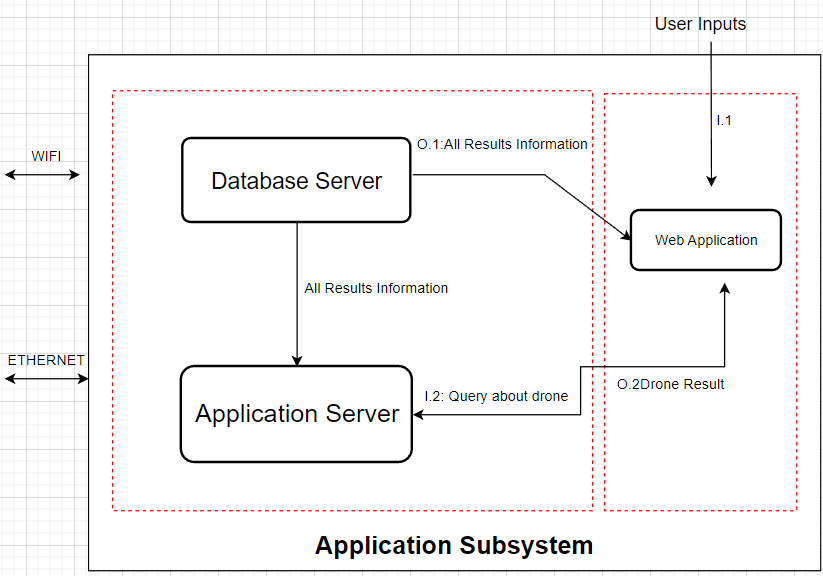
\includegraphics[width=0.70\textwidth]{images/Application_Subsystem.png}
 \caption{Data flow of Application Subsystem}
\end{figure}

\subsubsection{Assumptions}
For the operation of this subsystem, it is assumed that the user has access to WIFI or some form of internet and a browser to launch the web application.

\subsubsection{Responsibilities}
This subsystem is responsible for the database interaction with the user. First of all, the data of all the detected drone is displayed to the user then if the user requests for more information on a particular drone then the request is forwarded to the database in form of a query and the database results are displayed. 

\subsubsection{Subsystem Interfaces}

\begin {table}[H]
\caption {Subsystem interfaces} 
\begin{center}
    \begin{tabular}{ | p{1cm} | p{6cm} | p{3cm} | p{3cm} |}
    \hline
    ID & Description & Inputs & Outputs \\ \hline
    \#I.1 & User Inputs & \pbox{3cm}{Click on particular drone title} & \pbox{3cm}{Query to the database about the drone}  \\ \hline
     \#I.2 & Query about drone & \pbox{3cm}{The query to the database} & \pbox{3cm}{Results according to the query}  \\ \hline
    \#O.1 & List of objects & \pbox{3cm}{N/A} & \pbox{3cm}{List of drone and non drone objects}  \\ \hline
    \end{tabular}
\end{center}
\end{table}\subsection{Results Page}
The results page includes the output of the drones detected in the area which is presented to the user in graphical form. 


\begin{figure}[h!]
	\centering
 	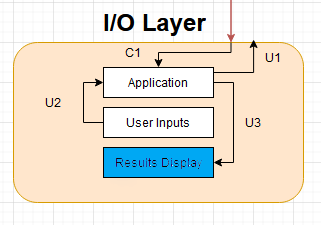
\includegraphics[width=0.60\textwidth]{images/results.png}
 \caption{Results Display Subsystem Diagram}
\end{figure}

\subsubsection{Assumptions}
The results page will only be online after the system is turned on.

\subsubsection{Responsibilities}
The responsibility of the results page is to communicate with the database through the application interface to provide the graphical visualization of the location of the system and any drones detected in the surrounding area. The results page will display the location of the device in the form of circular dot and any detected drones will be shown in triangular shape.

\subsubsection{Results Subsystem Interfaces}

\begin {table}[H]
\caption {Results interfaces} 
\begin{center}
    \begin{tabular}{ | p{1cm} | p{5cm} | p{4cm} | p{4cm} |}
    \hline
    ID & Description & Inputs & Outputs \\ \hline
    \#U3 & Communication with application & \pbox{4cm}{detected drones and system location data from the database} & \pbox{4cm}{Graphical view of the detected drones and location of the system}  \\ \hline
   
    \end{tabular}
\end{center}
\end{table}

\subsection{User Inputs}
The User Inputs page includes the input that can be taken from the user. Here, the user can select a detected drone and verify that it is a false positive. Also, user can select an individual drone and the system will actively track the selected drone in as close to real time as possible.


\begin{figure}[h!]
	\centering
 	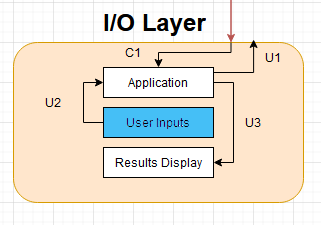
\includegraphics[width=0.60\textwidth]{images/userInputs.png}
 \caption{User Inputs subsystem diagram}
\end{figure}

\subsubsection{Assumptions}
The user can only select one drone at a time for active detection.

\subsubsection{Responsibilities}
The responsibility of the User Inputs is to provide a user interface to the user where they can select a detected drone and verify that it is a false positive. Also, the user can select an individual drone and the system will actively track the selected drone in as close to real time as possible.

\subsubsection{User Inputs Subsystem Interfaces}

\begin {table}[H]
\caption {User Inputs Subsystem interfaces} 
\begin{center}
    \begin{tabular}{ | p{1cm} | p{5cm} | p{5cm} | p{5cm} |}
    \hline
    ID & Description & Inputs & Outputs \\ \hline
    \#U201 & Single Drone Active Tracking & \pbox{5cm}{Select input from the user} & \pbox{5cm}{Selected Drone highlighted and actively tracked}  \\ \hline
    \#U202 & False Positive in detected Drones  & \pbox{5cm}{Select input from the user} & \pbox{5cm}{The selected object will not be further tracked}  \\ \hline
    \end{tabular}
\end{center}
\end{table}

\newpage

%%% References
\bibliographystyle{plain}
\bibliographystyle{reference/IEEEtran_custom}
\bibliography{reference/refs}{}

\end{document}